% Template for PLoS
% Version 1.0 January 2009
%
% To compile to pdf, run:
% latex plos.template
% bibtex plos.template
% latex plos.template
% latex plos.template
% dvipdf plos.template

\documentclass[10pt]{article}

% amsmath package, useful for mathematical formulas
\usepackage{amsmath}
% amssymb package, useful for mathematical symbols
\usepackage{amssymb}

% graphicx package, useful for including eps and pdf graphics
% include graphics with the command \includegraphics
\usepackage{graphicx}

% cite package, to clean up citations in the main text. Do not remove.
\usepackage{cite}

\usepackage{color} 

% Use doublespacing - comment out for single spacing
%\usepackage{setspace} 
%\doublespacing


% Text layout
\topmargin 0.0cm
\oddsidemargin 0.5cm
\evensidemargin 0.5cm
\textwidth 16cm 
\textheight 21cm

% Bold the 'Figure #' in the caption and separate it with a period
% Captions will be left justified
\usepackage[labelfont=bf,labelsep=period,justification=raggedright]{caption}

% Use the PLoS provided bibtex style
\bibliographystyle{plos2009}

% Remove brackets from numbering in List of References
\makeatletter
\renewcommand{\@biblabel}[1]{\quad#1.}
\makeatother


% Leave date blank
\date{}

\pagestyle{myheadings}
%% ** EDIT HERE **


%% ** EDIT HERE **
%% PLEASE INCLUDE ALL MACROS BELOW

%% END MACROS SECTION

\begin{document}

% Title must be 150 characters or less
\begin{flushleft}
{\Large
\textbf{Title}
}
% Insert Author names, affiliations and corresponding author email.
\\
Author1$^{1}$, 
Author2$^{2}$, 
Author3$^{3,\ast}$
\\
\bf{1} Author1 Dept/Program/Center, Institution Name, City, State, Country
\\
\bf{2} Author2 Dept/Program/Center, Institution Name, City, State, Country
\\
\bf{3} Author3 Dept/Program/Center, Institution Name, City, State, Country
\\
$\ast$ E-mail: Corresponding author@institute.edu
\end{flushleft}

% Please keep the abstract between 250 and 300 words
\section*{Abstract}
From nearly non-existence in the early 2000s, data breaches have exploded in terms of number of events and cumulative loss. As personal information has become the {\it ore} resource, mined by an Internet economy, which is largely based on targeted advertisement, there shall be no surprise that criminals steal and exploit personal data in their own way, such as for identity frauds. As people and organizations increasingly suffer their consequences, data breaches also undermine long-term confidence on the Internet as a reliable communication means, as good place for trustworthy data storage, and as a place in which a decent level of privacy can be maintained.



We conduct an exhaustive statistical analysis of data breaches as a new and fast evolving extreme risk, which has appeared and developed along with the Internet over a short period of nearly 15 years. In particular, we study (i) the evolution of the nature of the tail distribution over this period, (ii) the dynamics of the cumulative number of events and loss, and (iii) the improvements of event reporting and the completion of the catalog over time. Our results suggest that data breach cumulative loss has accelerated much faster than the total population of Internet users.

Based on the thorough assessment of dynamics and regularities, and taking into account the limitations of our study, we conduct out-of-sample predictions, and thus, provide some alarming forecasts concerning the evolution of data breach risk in the near future (5-year horizon).


% Please keep the Author Summary between 150 and 200 words
% Use first person. PLoS ONE authors please skip this step. 
% Author Summary not valid for PLoS ONE submissions.   
%\section*{Author Summary}

\section*{Introduction}
From nearly non-existence in the early 2000s, data breaches have exploded in terms of number of events and cumulative loss. As personal information has become the {\it ore} resource, mined by an Internet economy, which is largely based on targeted advertisement \cite{}, there shall be no surprise that criminals steal and exploit personal data in their own way, such as for identity frauds \cite{}. As people and organizations increasingly suffer their consequences, data breaches also undermine long-term confidence on the Internet as a reliable communication means, as a good place for trustworthy data storage, and as a place in which a decent level of privacy can be maintained.

The way people, organizations and governments shall view data breaches depends heavily on the risk they represent in terms of loss per event. In 2010, building on a dataset of 956 events, Maillart and Sornette showed that the distribution of severity, in terms of number of personal data loss per event, exhibited a power law tail distribution with an exponent $\mu \approx 0.7$ \cite{maillart2010}. With the information available at the time, the distribution was qualified of ``wild", according to Beno�t Mandelbrot, because neither its mean nor standard deviation were as a result of $\mu < 1$.

In the meantime, the number of records has been roughly multiplied by 10, with 9,576 exploitable events as of 31/10/2014. Also, the rate of events, as well as the cumulative loss, have tremendously accelerated (increased?) as shown on Figure \ref{dynamics}. We shall therefore re-define the nature of data breach risk in light of cumulative information made available breach after breach, in order to outline a predictive model for a major extreme risk that has emerged less than 15 years ago.

{\bf Outstanding questions}
\begin{itemize}
  \item What drive the exponential growth of cumulative loss? Is it due to the exponential  increase of events, or as a result of the nature of the distribution of loss?
  \item Has the risk worsened over time, or do we only witness an unravelling process of emerging risks?
  \item Estimate maximum loss ?
  \item 
\end{itemize}


After presenting the data (Section \ref{}), we determine the nature and the stability of the tail distribution using a novel approach \cite{}, combining the Generalized Extreme Value (GEV) \cite{} and the Generalized Pareto Distributions GPD) \cite{} theories (Section \ref{}),.We then analyze the exponential dynamics of events and cumulative loss, and how our understanding of the tail distribution helps establish a functional relation between the dynamics of events and loss (Section \ref{}). These results are crucial to model the return time of events of a given size. This {\it return-time} measures are typically used by civil engineers for designing infrastructures with a sufficient safety level to cope with large natural disasters, such as floods \cite{}, earthquakes \cite{}, hurricanes \cite{}, or by the insurance industry to calculate insurance premiums, capital reserves, and coverage limits. Similarly, {\it return-time} should be the cornerstone measures for designing sufficient safety measures to prevent cyber attacks, and to provision sufficient capital reserves to cope with a data breach event.

\section*{Data}
\section*{Exponential Dynamics}
Unlike other widely studied risks, the specificity of data breaches from a statistical perspective is the increase rate of event occurrence. 

We will see later that these dynamics impact tremendously statistical forecasting of event return times, as well as our growing understanding of data breach risks, through catalog completion.




\section*{Distribution}

In earthquake, assumption that there is limit beyond which no earthquake is observed, vs ``soft" truncation

in earthquake, earthquakes occurrence and magnitudes can be related to the structure and dynamics of the earth crust. For data breaches, it is a function of user base size and data quality/value, IT security, which determine the incentives for cyber criminals to spend time, money and expertise resources on attacks. Unfortunately, this very function is unknown, but we know that a company cannot suffer a loss larger than the amount of its user data assets.

Figure \ref{distribution} shows a distribution, which exhibits a power law distribution truncated for both small and large events. The lower cutoff can be attributed to the incapacity to record small events {\bf (see SI for more details on how this threshold has lowered as more events could be recorded and reported)}. As time passes, the upper threshold gets more pronounced, and quick visual estimation shows that $S_max \approx 2~10^8$. We shall refine this estimation by combining the GEV and GPD theorems underlying the Extreme Value Theory \cite{}.

\subsection*{Method Combining GEV and GPD}
Extreme Value Theory (EVT) studies the limiting distribution of maxima of identically independently distributed (iid) random variables (rv) as the sample size tends to infinity. Two main limit theorems constitute the basis for the application of EVT: (i) the main limit theorem of EVT (proved by Frechet \cite{} for Pareto-type limit distribution and by Fischer and Tippet \cite{} for Weibull and Gumbel distributions), leading to the Generalized Extreme Value (GEV) theory and (ii) the theorem by Gnedenko-Pickands-Balkema-Haan leading to the Generalized Pareto Distribution (GPD).

{\bf Tell shortly what GEV and GPD measure, then move details to SI}

\paragraph{Duality between the two main theorems of extreme value theory: }These two limit theorems show that information on the distribution of extreme events can be gathered in two ways: (i) by measuring the maximum of a sample whose size $n$ goes to infinity, or (ii) by recording the excess function $F_H(x)$ of that sample when increasing the threshold $H$ to its upper limit $x_F$.

\subsection*{Method}
All the ``trick" consists in evaluating the parameters of GEV and GPD for the ``right" time intervals $T$ and the right amplitude $H$ for which the limit FFT and GPBH theorems are (approximately) valid. We shall therefore calibrate the GEV and GPD models for resp. a variety of intervals and amplitudes. Additionally, we shall perform proper bootstrapping to ensure robustness (e.g., select intervals randomly for GEV? $\rightarrow$ check method Pisarenko and Sornette).















\section*{Discussion}

How is it the cumulative loss is only loosely related to the number of events? 
% Results and Discussion can be combined.
% You may title this section "Methods" or "Models". 
% "Models" is not a valid title for PLoS ONE authors. However, PLoS ONE
% authors may use "Analysis" 
\section*{Materials and Methods}

% Do NOT remove this, even if you are not including acknowledgments
\section*{Acknowledgments}


%\section*{References}
% The bibtex filename
%\bibliography{template}
\section*{Figures}


\begin{figure}[h]
\begin{center}
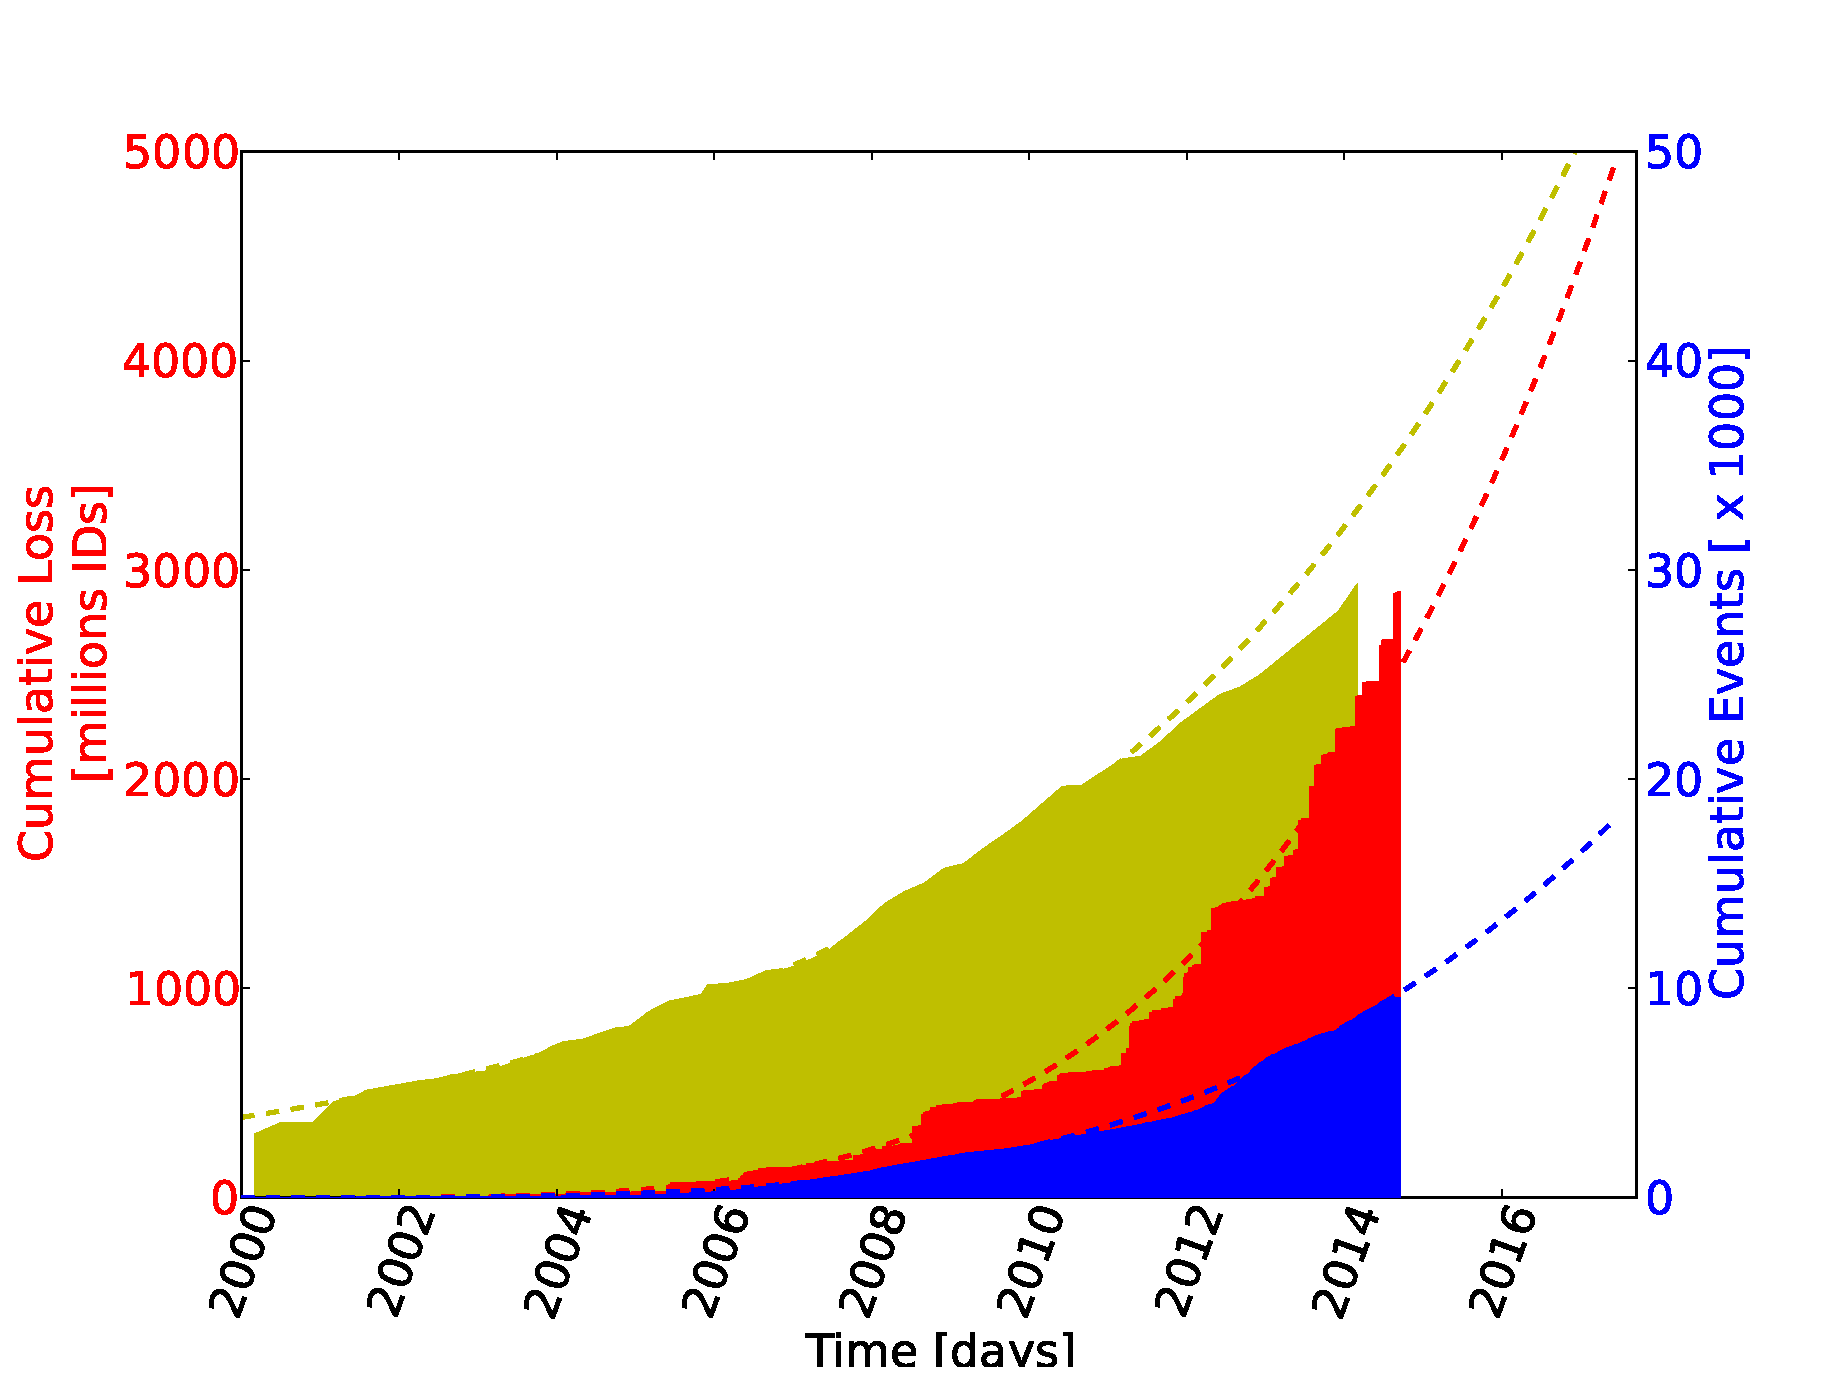
\includegraphics[width=6in]{../figures/dynamics.eps}
\caption{Evolution of cumulative number of events (blue) and cumulative loss (red). For comparison, the total number of Internet users is also reported (yellow) on the same scale as loss.}
\label{fig:dynamics}
\end{center}
\end{figure}


\begin{figure}[h]
\begin{center}
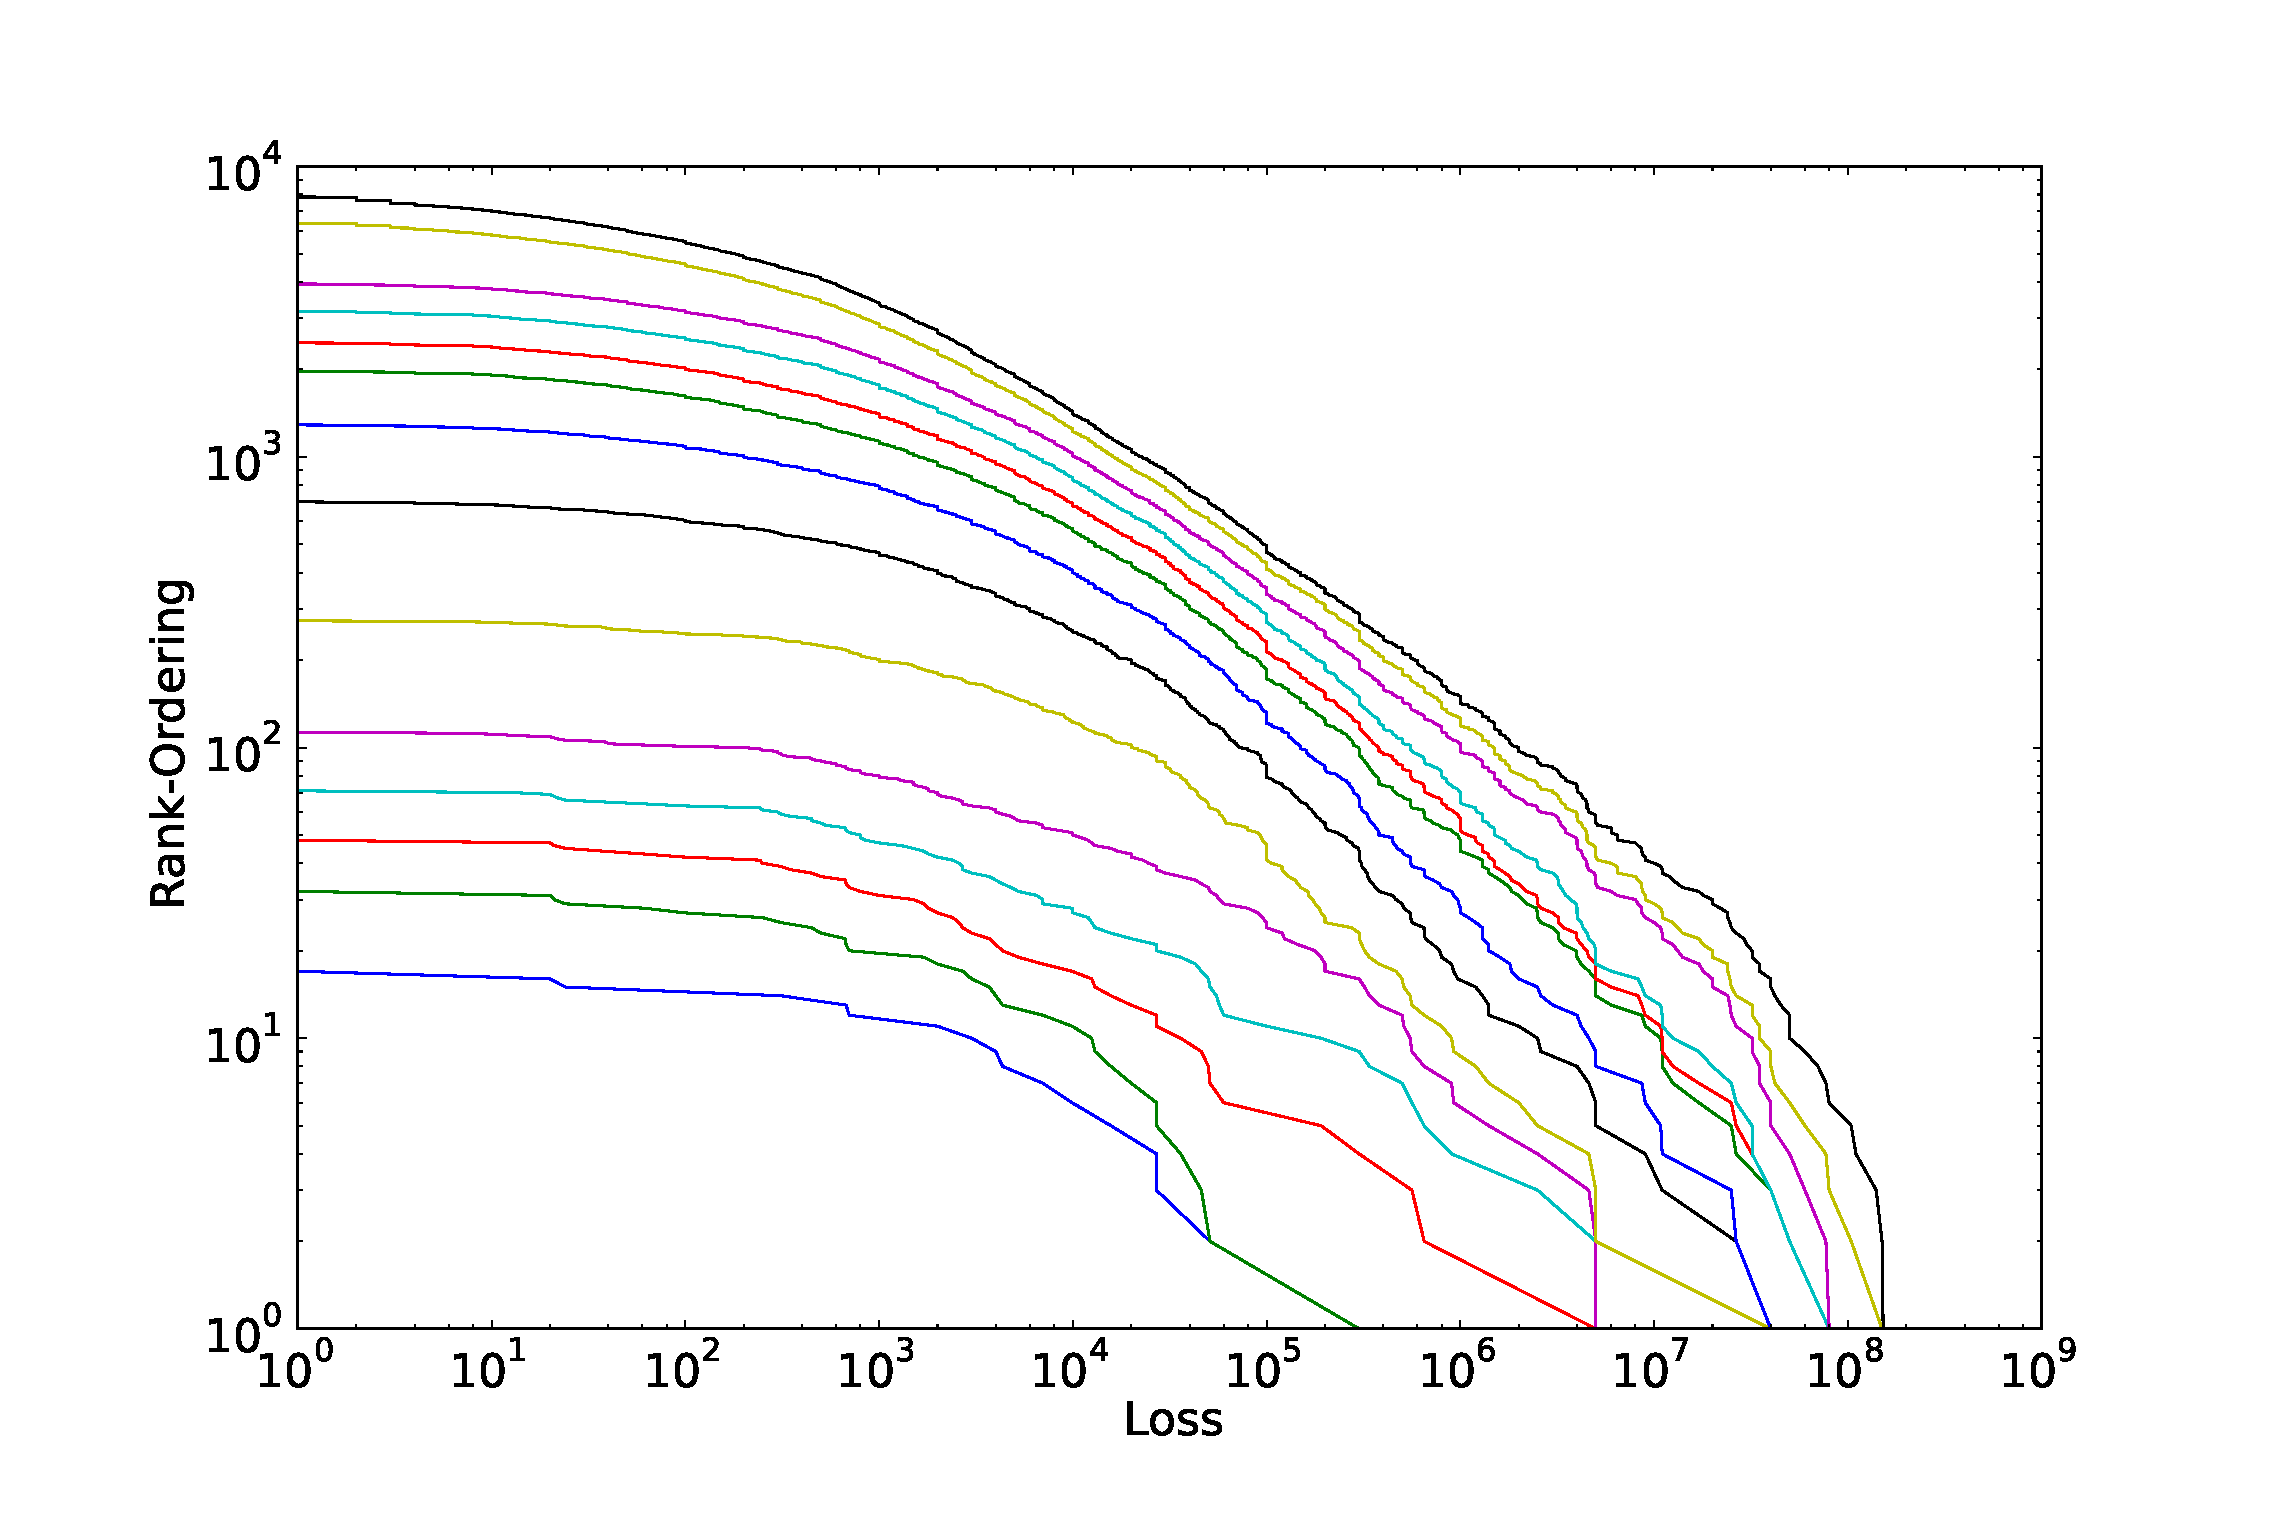
\includegraphics[width=6in]{../figures/CCDF.eps}
\caption{Evolution, year-by-year, of the Complementary Cumulative Distribution Function (CCDF), presented here in the form of a rank-ordering for convenience.}
\label{fig:dynamics}
\end{center}
\end{figure}


\clearpage
\begin{center}
{\bf \Huge Supplementary Materials}
\end{center}


\vspace{1cm}


\section{Data Collection and Catalog Structure}

\subsection{Time lag between event occurrence and reporting}

\begin{figure}[h]
\begin{center}
%\includegraphics[width=6in]{Figures/avg_classification_accuracy_per_subject.png}
\caption{Time lag between event occurrence and reporting}
\label{ }
\end{center}
\end{figure}

\subsection{Percentile of events over threshold over time}

\begin{figure}[h]
\begin{center}
%\includegraphics[width=6in]{Figures/avg_classification_accuracy_per_subject.png}
\caption{Percentile of events over threshold over time (moving window). (lower panel) number of events reported. Another way to design the figure would be to show the number of events in the 15th, 30th, 50th, 70th, 85th quantiles over time.}
\label{ }
\end{center}
\end{figure}

From Figure \ref{}, we clearly see that the increasing rate of events is mainly due to the reporting of small (and medium) events. This shall be explained by data sources, in particular, data concerning the Data Breach Notification Act (DBNA), and released by States under the Freedom of Information Act (FOIA).


\subsection{Catalog Completion}

In \cite{},  Maillart and Sornette suggested that the lower cut-off was the result of catalog incompletion. We shall verify this hypothesis, and characterize the evolution of the lower cut-off as a function of the rate of events.



\section{Estimation of Maximum Data Breach Magnitude using the combined GEV and GPD methods}




However, for events with magnitude larger than $M \approx 3.5$, and starting from 2005 ($t > 1825~days$), the rate remains roughly constant ($\lambda \approx 0.68$). We shall consider this subset of 2401 events to estimate the maximum magnitude $M_{max}$ in a given interval (rephrase).


\begin{figure}[h]
\begin{center}
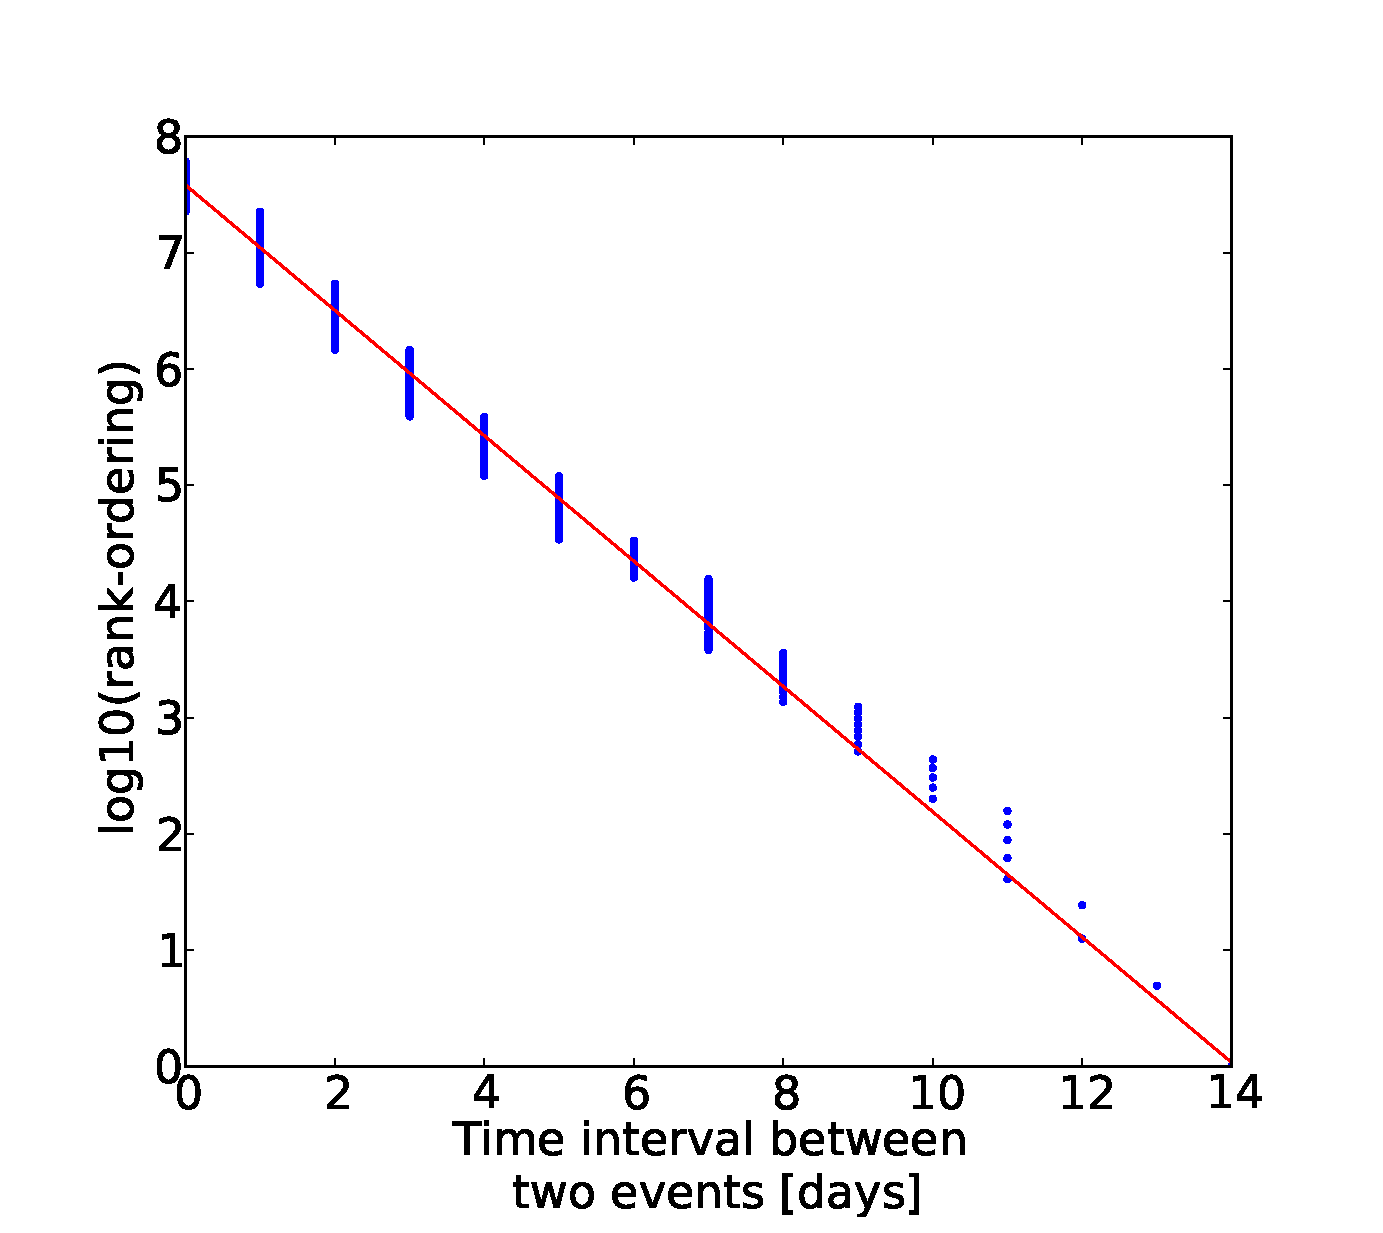
\includegraphics[width=4in]{../figures/SI/exponential_distribution.eps}
\caption{Distribution of rate of events of magnitude $M \geqslant 3.5$ and starting from 2005 ($t > 1825~days$). The straight line (red) in logarithmic y-scale and linear x-scale shows that the distribution of inter-time between two events is indeed exponential with $\lambda \approx 0.68$.}
\label{fig:exponential_rate}
\end{center}
\end{figure}




\begin{figure}[h]
\begin{center}
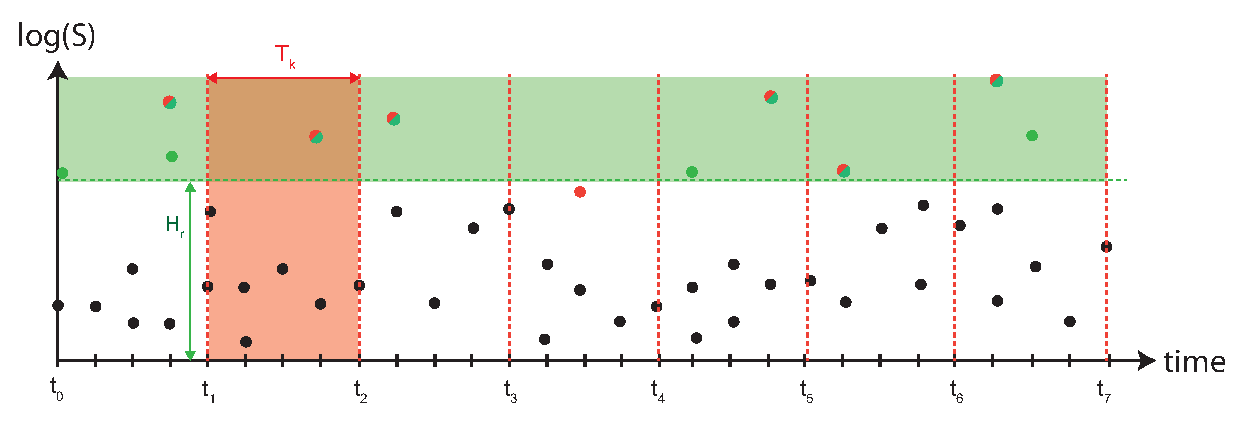
\includegraphics[width=6in]{../figures/SI/GEV_GPD_combined.eps}
\caption{Schematic of the combined GEV GPD method.}
\label{ }
\end{center}
\end{figure}






\subsection{Application of the GEV Method to the Data Breach catalog}


\subsection{Application of the GPD Method to the Data Breach catalog}

{\bf INSERT TABLE like {\it Table 18}}

\begin{enumerate}
  \item {\bf Choose the appropriate interval for T-values: } Kolmogorov distance + visual check ?
  \item 
  \item 
\end{enumerate}






%\section*{Tables}
%\begin{table}[!ht]
%\caption{
%\bf{Table title}}
%\begin{tabular}{|c|c|c|}
%table information
%\end{tabular}
%\begin{flushleft}Table caption
%\end{flushleft}
%\label{tab:label}
% \end{table}

\end{document}

